\documentclass{beamer}
%------------------Math Setup-------------------

%%% Packages

\usepackage{amsmath}        % math environments
\usepackage{mathtools}      % tools for math formating
\usepackage[nice]{nicefrac} % nicer fractions
\usepackage{cancel}         % allows to scratch expressions.
\usepackage{slashed}        % allows to slash individual characters.
\usepackage{xargs}          % better handling of optional arguments for commands
\usepackage{braket}         % convenient Dirac notation

%%% Custom macros

\usepackage{macros} % custom latex macros (macros.sty)

%------------Fonts (Body and math)--------------

%%% Main font (EB Garamond)

\usepackage{fontspec} % Finer font selection (requires Lua/XeLaTeX)
\setmainfont{EB Garamond}[
  Ligatures   = TeX, % ligatures
  OpticalSize = On, % optical weight adjustment
  % Numbers     = OldStyle, % can be a little hard to read
  SmallCapsFeatures = {LetterSpace=5} % Adds spaces for small caps
]

%%% Math font (Libertinus Math)

\usepackage{unicode-math} % Finer math font selection
\setmathfont{Libertinus Math}[ % Nice neutral universal math font
    Scale=MatchLowercase
]
\setmathfont[ % Adding back a familiar mathcal
    range = {\mathcal, \dagger, \ddagger},
    Scale = MatchLowercase
]{Latin Modern Math}

%-----------------Misc packages-----------------

\usepackage[french]{babel} % language support
\usepackage{setspace} % line spacing
\usepackage{cite} % in text citations
\usepackage{microtype} % small typography tweaks
\usepackage{graphicx}		% figure insertion
\usepackage{subfig}			% allows for subfigures
\usepackage{geometry}		% document geometry
\usepackage{fancybox}		% boxes, frames etc
\usepackage{url}            % typographically sound URLs
\usepackage{float} % Fixes hacky geometry problems
\usepackage[
format    = hang,
margin    = 5mm,
font      = small,
labelfont = bf,
labelsep  = space
]{caption} % tweak caption layout and format
\usepackage{csquotes} % For quotes
\newcommand\itsym{$\bullet$} % symbole pour les listes

%--------------------Tables---------------------

\usepackage{array} % tabular functions
\newcolumntype{C}{>{$\displaystyle}c<{$}} % centered math column
\newcolumntype{L}{>{$\displaystyle}l<{$}} % left aligned math column
\newcolumntype{R}{>{$\displaystyle}r<{$}} % right aligned math column
\renewcommand{\arraystretch}{1.5} % vertical spacing of tables
\usepackage{dcolumn} % allows for aligning of values wrt to the decimal
\addto\captionsfrench{\renewcommand\frenchtablename{{\FBfigtabshape Tableau}}} % rename table name (french)

%---------------General layout------------------

\usepackage{theme/layout}

%-------------Colors and Hyperref---------------

% Pass hyperref options before loading pdfx
\PassOptionsToPackage{
    backref=page,
    pagebackref=true,
    hyperindex=true,
    bookmarks=true,
    pdfa
}{hyperref}

\usepackage[a-2b,mathxmp]{pdfx}[2018/12/22] % ???

% options PDF
\hypersetup{
    colorlinks=true,         % colorise les liens
    breaklinks=true,         % permet le retour la ligne dans les liens trop longs
    urlcolor=URLColor,       % couleur des hyperliens (doit inclure x11names dans xcolor ci-dessus)
    linkcolor=LinkColor,     % couleur des liens internes
    citecolor=CiteColor,     % couleur des liens de citation
    bookmarksopen=true,      % ouvre les signets PDF au départ
}

%%% Choose color theme

\usepackage{colorthemes/colors_marine} % choose a style

%%% Colored boxes

\usepackage{empheq}
\setlength{\fboxrule}{1pt} % sets the border width globally (or locally in a group)
\setlength{\fboxsep}{4pt}  % sets padding between frame and content

% \usepackage{tcolorbox}
% \tcbuselibrary{theorems}
% \tcbset{%
%     highlight math style={
%         colframe=MainColor, % MainColor defined in colorthemes
%         colback=white,
%         arc=4pt,
%         boxrule=1pt,
%         sharp corners
%     }
% }

% % Use a colored box for 'cboxed'

% \newcommand{\cboxed}[1]{\tcbhighmath{#1}}


%-------------------------------------------------------------------------------
% Figures TiKz !!!TODO FIX THIS!!!
\usepackage{tikz}
\usetikzlibrary{
	calc,
	patterns,
	positioning,
    external,
    shapes,
    fit,
    backgrounds,
    arrows.meta,
	positioning,
    decorations,
    decorations.pathmorphing,
    decorations.markings,
    shapes.geometric,
    arrows
}
\tikzexternalize[prefix=figures/pdf/]

\usepackage{pgfplots}
\pgfplotsset{compat=1.16}
\pgfdeclarelayer{background}
\pgfdeclarelayer{foreground}
\pgfsetlayers{background,main,foreground}

\usepackage{theme/tikzstyles}
%%%%%%%%%%%%%%%%%%%%%%%%%%%%%%%%%%%%%%%%%%%%%%%%%%%%%%%%%%%%%%%%%%%%%%%%%%%%%%%%


\title[Short title]
{A sample presentation}
\subtitle{With ramblings from a madman}
\author{Théo N. Dionne}

\institute[]{
    APS March Meeting \\
    Denver Colorado \\
    \today
}

\date{} % suppress date field

\titlegraphic{
    \includegraphics[width=3cm]{./figures/logos/UdeS_logo_h_noir_cropped.pdf}
    \hspace{1cm}
    \includegraphics[width=4cm]{./figures/logos/IQ_logo_h_noir_cropped.pdf}
}

\begin{document}

\begingroup\setbeamertemplate{navigation symbols}{}

\begin{frame}[noframenumbering]
	\titlepage
\end{frame}


\begin{frame}[noframenumbering]\frametitle{Table of contents}
    \tableofcontents
\end{frame}

\endgroup

\begin{frame}
\frametitle{Title}
The quick brown fox jumps over the lazy dog \cite{hubbardI}.
\pause
\al{\cboxed{
    i\hbar\del_t\ket{\Psi} = \op{H}\ket{\Psi}
}}
\end{frame}

\section{A section}
\subsection{A subsection}
\begin{frame}
\frametitle{What}\pause
\begin{itemize}
	\item One.\pause
	\item Two.\pause
	\item Three.
\end{itemize}
\end{frame}
\subsection{Another subsection}
\begin{frame}\frametitle{The state of the world}
\begin{theorembox}{Birb}{thm:birb}
	Birbs exist.
\end{theorembox}
\end{frame}

\begin{frame}\frametitle{Colorbox test}
\begin{highlightcbox}
	\begin{center}
	    A very important result.
	\end{center}
\end{highlightcbox}
\end{frame}

\begin{frame}\frametitle{A test of what the box environment looks like}
    \begin{cbox}
    This is the fundamental theorem of calculus:
    \al{
        \int_{a}^{b}f(t)\,\D{t} = F(b) - F(a)
    }\pause
    Notice:
    \begin{itemize}
        \item thing to say;\pause
        \item another thing to say;\pause
        \item consider $\ve{F} = m\ddot{\ve{x}}$.
    \end{itemize}
    \end{cbox}
\end{frame}

\begin{frame}\frametitle{A simple derivation}
    Extremization of the action entails:
    \ald{
        \cboxed{0 = \delta\mathcal{S}} &= \int_{t_i}^{t_f}\D{t}\,\delta\mathcal{L}\pause\\
        &= \int_{t_i}^{t_f}\D{t}\cro{\ddf[\mathcal{L}]{q}\delta{q} + \ddf[\mathcal{L}]{\mspace{1.5mu}\dot{q}}\delta\mspace{1.5mu}\dot{q}}\pause\\
        &= \int_{t_i}^{t_f}\D{t}\cro{\ddf[\mathcal{L}]{q} - \dd{t}\ddf[\mathcal{L}]{\mspace{1.5mu}\dot{q}}}\delta{q} + \underbrace{\int_{t_i}^{t_f}\D{t}\dd{t}\p{\ddf[\mathcal{L}]{\mspace{1.5mu}\dot{q}}\delta{q}}}_{\text{vanishes (B.C.s)}}\pause\\
        &\Rightarrow \cboxed{\ddf[\mathcal{L}]{q} - \dd{t}\ddf[\mathcal{L}]{\mspace{1.5mu}\dot{q}} = 0}\pause
    }
    The converse is equally true, hence:\pause
    \al{\highlightcboxed{
        \delta\mathcal{S} = 0 \text{ \& B.C.s} \Longleftrightarrow \ddf[\mathcal{L}]{q} - \dd{t}\ddf[\mathcal{L}]{\mspace{1.5mu}\dot{q}} = 0
    }}
\end{frame}

\begin{frame}\frametitle{Testing columns}
\begin{columns}
    \column{0.5\linewidth}
    This is a Woodcock. Its features are:
    \begin{itemize}
        \item<2-> A beak
        \item<3-> Wings
        \item<4-> A brain (barely)
        \item<5-> Camouflage
    \end{itemize}

    \column{0.5\linewidth}<1->
    \centering
    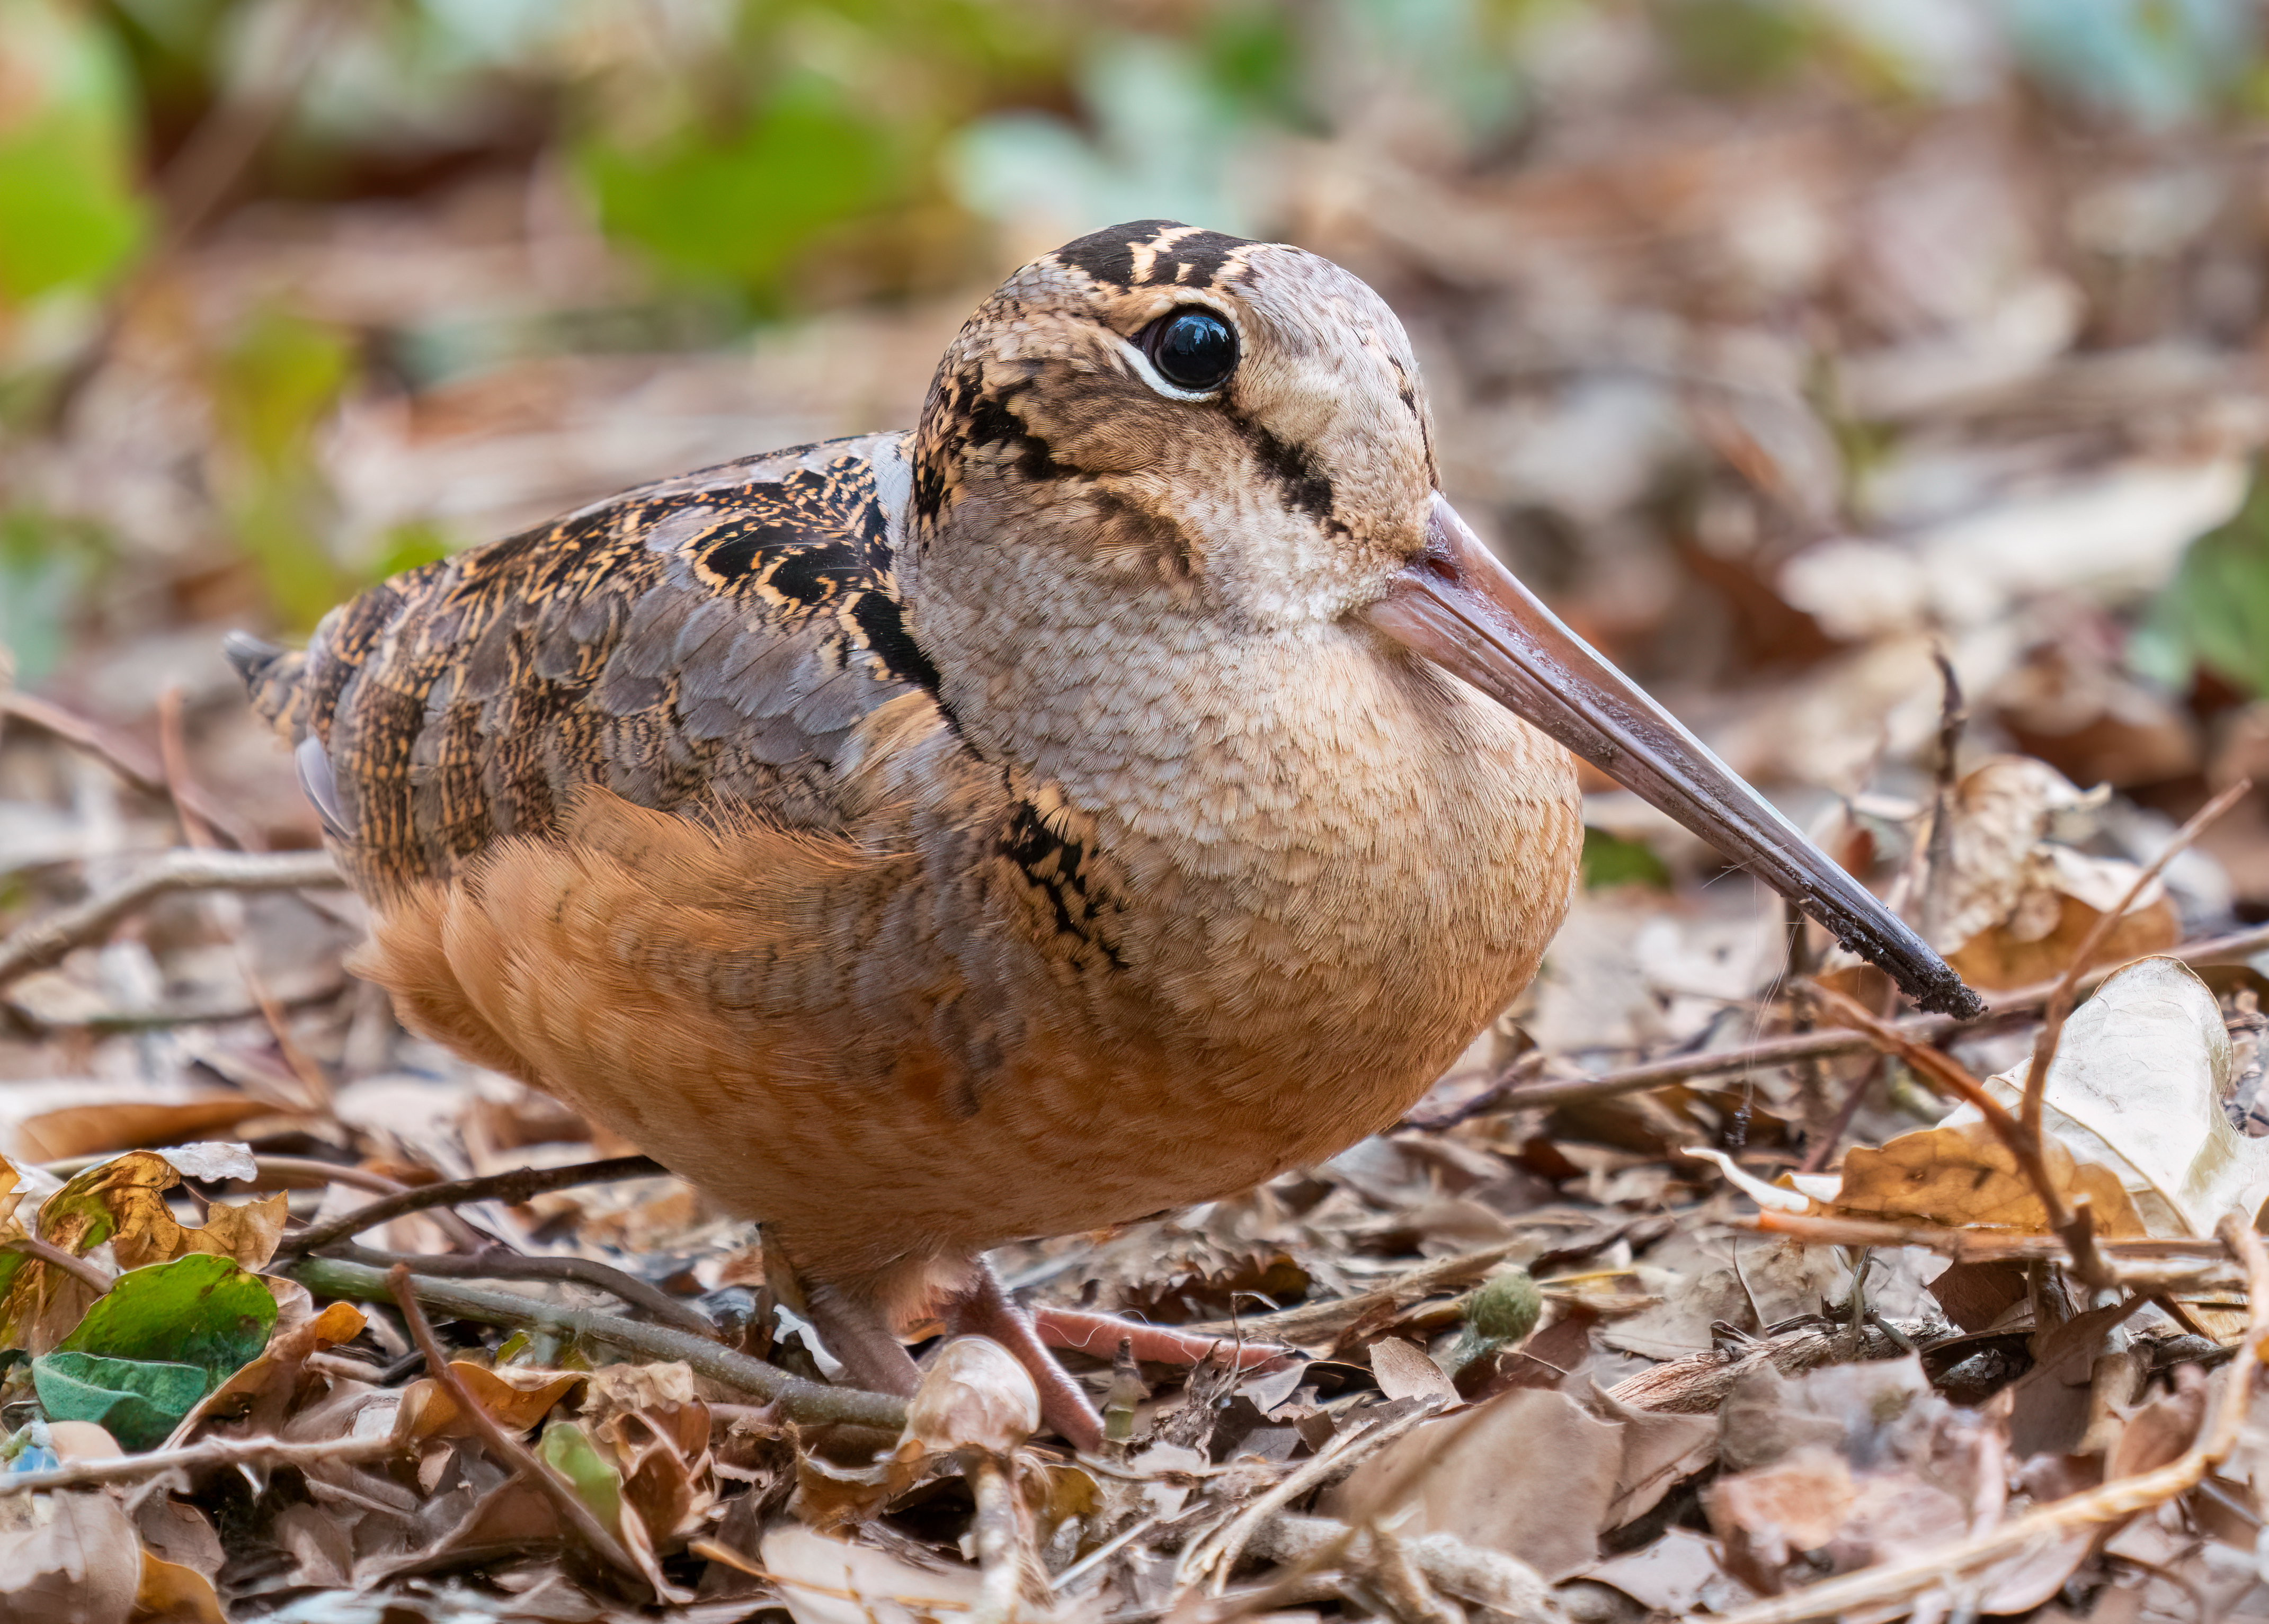
\includegraphics[width=\linewidth]{figures/American_woodcock.jpg}
\end{columns}
\end{frame}

\begin{frame}
	\begin{center}
		\vfill\vspace{1em}
		    \Huge \sffamily \bfseries \color{MainColor} Questions (2 minutes)
		\vfill
	\end{center}
\end{frame}

\begin{frame}
\begin{center}
\begin{beamercolorbox}[sep=1em, center]{frametitle}
  {\usebeamerfont{title}Thank You!}
\end{beamercolorbox}
\end{center}
\end{frame}

\begin{frame}[allowframebreaks]\frametitle{Bibliography}
\singlespacing
\nocite{*} % Shows all references regardless of if cited
\bibliographystyle{CodexStyle/bibstyles/nature-fr} % Use "nature" for english version
% \addcontentsline{toc}{chapter}{Bibliographie} % Add bibliography
\bibliography{These}
\end{frame}

\end{document}
